\chapter{Revisão bibliográfica} \label{chap:revBibli}
	\section{Breve revisão dos conceitos utilizados neste trabalho}

		\subsection{Redes neurais convolucionais}
			\par Um dos classificadores usados nesse trabalho é baseado na tecnologia de redes neural as convolucionais, Das redes tem como principal característica a convolução aplicada aos dados de entrada segundo um segundo um "kernel", Nesse caso entende-se "kernel"Como uma série de valores que deve ser aplicados valor a valor Afim de preparar os dados para classificação de uma rede neural densa, no caso específico das redes neurais convolucionais Essa série de valores que serviram como filtro da entrada da rede neural convolucional, Na verdade, É apenas a aplicação da função de ativação em cada valor, Ou seja, se a função de ativação escolhida for a sigmóide, Aplicar-se-á Esta função a cada valor de entrada da rede, caso a função de ativação seja a Relu O mesmo será feito \cite{UYCNWV}.
			
			\par A aplicação do \textit{kernel} também pode ser feita da seguinte forma: soma se os valores vezes seus respectivos pesos e aplica-se a função de ativação.
			
			\par Um aspecto importante da preparação dos dados para treinamento chama-se \textit{padding} Que consiste no aumento do vetor de entrada para que o vetor de saída tenha sempre o mesmo tamanho que o vetor de entrada.
			Em redes convolucionais O resultado terá sempre um número menor de itens do que a entrada, assim, é preciso adicionar zeros no início ou fim do vetor de entrada ou apenas no início (recomendado no caso de realização de previsões).

			\par O \textit{stride} ou passo é outro fator que influencia no tamanho da saída de uma convolução. O Passo é a quantidade de deslocamentos que uma janela de convolução deve realizar quando necessita avançar no vetor fornecido, quanto maior o passo menos valores serão fornecidos como resultado aumentando assim a necessidade de \textit{padding} caso se necessite manter o tamanho do vetor de entrada para a próxima camada.Dependendo da fase da convolução, esse encurtamento necessário e desejável pois pode revelar padrões cujos os ruídos impediam de serem vistos.
			
			\par TODO: Ver \textit{wavenets no notebook}
			
			\par \cite{CNNC}

		\subsection{Treinamento e particionamento da série de dados}
			\par Quando do treinamento de uma rede necessitas-se Que os dados usados para tal fim sejam particionados, Para tal, é necessário separar os dados em uma partição de treinamento,Outra de validação, e finalmente uma de teste.

		\subsection{Funções de ativação}
			\par As funções de ativação geralmente são aquelas cujo resultado varia entre -1 e 1 ou entre 0 e 1 caso sejam saturáveis como as \textit{hiperbólicas} e \textit{sigmoides} ou entre em zero e infinito como é o caso da \textit{Relu} caso sejam não saturáveis.
		\subsection{Funções de erro}
			\par As funções de erro são usadas para computar a diferença entre os valores produzidos pelo modelo e os valores, de fato, desejados, dependendo dos resultados desejados se pode usar uma ou outra função de erro, na listagem abaixo estão descritas algumas funções de erro e seus usos recomendados.

			\begin{itemize}
				\item $erros = previsao - desejado  \qquad \rightarrow$ : Erro simples, não destaca nem suprime nenhuma característica.
				\item $mse = \dfrac{1}{n}*\sum_{n=1}^{tamanho} erros[n]^2 \qquad \rightarrow$ Média dos quadrados dos erros: Usada quando é necessário destacar os de maior valor. Então se o custo de erros grandes é importante para aplicação esta função é recomendada.
				\item $mae = \dfrac{1}{n}*\sum_{n=1}^{tamanho} |erros[n]| \qquad \rightarrow$ Média dos valores absolutos: Usada quando os resultados são proporcionais ao erro.
				\item $mape =  \dfrac{1}{n}*\sum_{n=1}^{tamanho} |erros[n] / desejado[n]| \qquad \rightarrow$ Média da percentagem de erro absoluto: Informa o tamanho do erro comparado com o valor desejado.
			\end{itemize}

		\subsection{Técnicas de treinamento de redes}
		
			\subsubsection{Parada antecipada de treinamento}
				\par A técnica de parada antecipada de treinamento pode ser usada quando a rede neural por algum tempo pára de convergir, dessa forma é possível evitar o gasto desnecessário de processamento quando a rede pára de convergir. Esta técnica também ajuda a rede a evitar um \textit{overffiting}.

		\subsection{Redes neurais residuais}

		\begin{figure}[H]
			\centering
			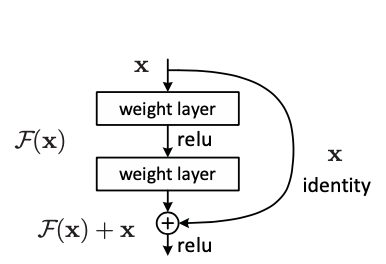
\includegraphics[width=0.7\linewidth]{images/ResidualLearnningBuildBlock}
			\caption[Residual learning: a building block.]{Residual learning: a building block.}
			\label{fig:residuallearnningbuildblock}
		\end{figure}
	
		\par De acordo com \cite{DBLP:journals/corr/HeZRS15} Redes neurais residuais são aquelas que "pulam" algumas camadas, ou seja, a saída de uma camada vai para a próxima mas também vai para uma outra mais à frente. 
		\begin{figure}
			\centering
			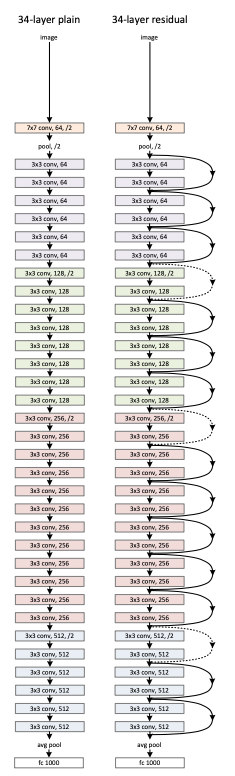
\includegraphics[width=0.3\linewidth]{images/ResidualLearnningNNAndRegularNN}
			\caption[Comparação entre uma rede neural regular e uma rede neural residual]{Comparação entre uma rede neural regular e uma rede neural residual, a direita a rede neural regular percorre sequencialmente todas as suas camadas, a esquerda a rede neural residual "pula" algumas camadas reiteradamente.}
			\label{fig:residuallearnningnnandregularnn}
		\end{figure}
		
		
		
		\subsection{Sinais digitais e sub-amostragem (\textit{downsampling})}
			
		\subsection{Caracterização dos processos de produção da voz humana}
		
	\section{Estado-da-arte em \textit{Imagined Speech}}